\scanpage{101}
\mspage{18}
\margin{Moreover, one should require \unsure{1°} that $\Theta$ be trivial on $I'\cap X'_K$, and that a power $\Theta^{\unsure{\nu K}}$ of $\Theta$ $(\nu\geq1)$ be \unsure{trivial|trivial} 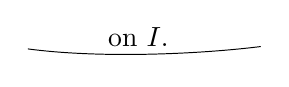
\begin{tikzpicture}[baseline=(surI.base),line cap=round]
\node[inner sep=0pt] (surI) at (0,0) {on $I$.};
\draw[line width=.35pt] (-1.40,-.15)
 ..controls(-.50,-.27)and(.74,-.22)..(1.55,-.12);
\end{tikzpicture} For $X'_K\ne\phi$ then implies that $X'$ is $\unsure{+}$, $\unsure{=}$ connected. \deleted{Moreover}}

of $\Theta$ lifts to an action of $\Theta$ on $\widehat{\Pi}_1(X',I')$, where $I'=X'\vert I$.
\deleted{$\unsure{\exists a'\in}$} $I'\cap X'_K\ne\phi$, $X'$ \unsure{being|being} connected (it suffices that $\Gamma$ be transitive on $\pi_0(X')$ i.e. that $X'$ be ``$K$-connected'' i.e. connected as a scheme over $K$) so the lifted action is unique.

\inserted{Condition 2 is made explicit in practice as a stability condition for certain open subgroups of a $\pi_1(X,x)$ $(x\in X_K\cap I)$ under the action of $\pi$}

3) Under the conditions of 2), for every homomorphism $f:X'\longrightarrow Y$ and \deleted{every}\inserted{an} $x'\in X'_K\cap I'$, \deleted{the action} can find the $\Theta'$ \deleted{\unsure{of such}} in such a way that the automorphism of $\widehat{\pi}_1(X',x')$ which it induces leaves invariant the kernel of
\[
\widehat{\pi}_1(X',x)\mathrel{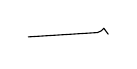
\begin{tikzpicture}[baseline=-.35ex,line cap=round,line join=round]
\draw[line width=.4pt] (0,0)--(.88,.055)
 ..controls(.92,.06)and(.94,.09)..(.96,.11)--(1.015,.035);
\end{tikzpicture}}\widehat{\pi}_1(Y,f(x)).
\]
This is again a stability condition for certain subgroups, but not necessarily of finite index, of $\pi_1(X,x)$ under $\Theta$.

\margin{One can \deleted{\unsure{generalize}}\inserted{strengthen} this condition, by \unsure{by assuming|assuming} \deleted{\unsure{every|$\forall$}} \unsure{not} that $x'\in X'_K\cap I$, and by \deleted{\unsure{imposing it}} requiring that for every $\nu$ such that $\Theta'^\nu x'=x'$, $\Theta'^\nu$ on $\pi_1(X',x')$, \unsure{preserves the kernel of} $f$ $\widehat{\pi}_1(Y,f(x'))$.}

4) Let $X'_1,X'_2$ be two finite étale coverings of $X$, and $f$ a morphism
\[
X'_1\xrightarrow{f}X'_2
\]
(\uuline{not necessarily} \uuline{an $X$-morphism} !), $I'_1=X'_1\mathrel{\begin{tikzpicture}[baseline=-.50ex,line cap=round]
\draw[line width=.4pt] (0,-.17)--(0,.21);
\draw[line width=.4pt] (0,0)--(.10,.01);
\end{tikzpicture}} I$, $I'_2=X'_2\vert I$ we assume \deleted{already that} that $J\overset{\mathrm{def}}=I'_1\cap f^{-1}(I'_2)\ne\phi$, \deleted{more precisely that} \deleted{$\unsure{I'_1|X'_1}\cap f^{-1}(I'_2)\longrightarrow$} then \deleted{the morphism} the morphism
\[
\Pi_1(X'_1,J)\longrightarrow\widehat{\Pi}_1(X'_2,I'_2)
\]
is compatible with the action 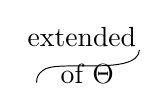
\begin{tikzpicture}[baseline=(deTheta.base),line cap=round]
\node[anchor=base west,inner sep=0pt] (deTheta) at (.27,0) {of $\Theta$};
\node[anchor=base west,inner sep=0pt] (prolongee) at (-.15,.46) {\inserted{extended}};
\draw[line width=.35pt] ([xshift=1pt,yshift=-1pt]prolongee.south east)
 ..controls(1.25,.08)and(.20,.31)..(.05,.16)
 ..controls(-.01,.12)and(-.03,.07)..(-.03,.01);
\end{tikzpicture} on the groupoids (for a compatible choice of this action, if there is ambiguity, cf 2°).
\mspage{100}
